\chapter{Gestión del proyecto}

\section{Alcance}

\section{Análisis de requisitos}

\section{Análisis de riesgos}

\section{Análisis de costes}

\section{Gestión de la configuración}

\section{Planificación temporal}

\subsection{EDT}

\begin{figure}[H]
    \centerline{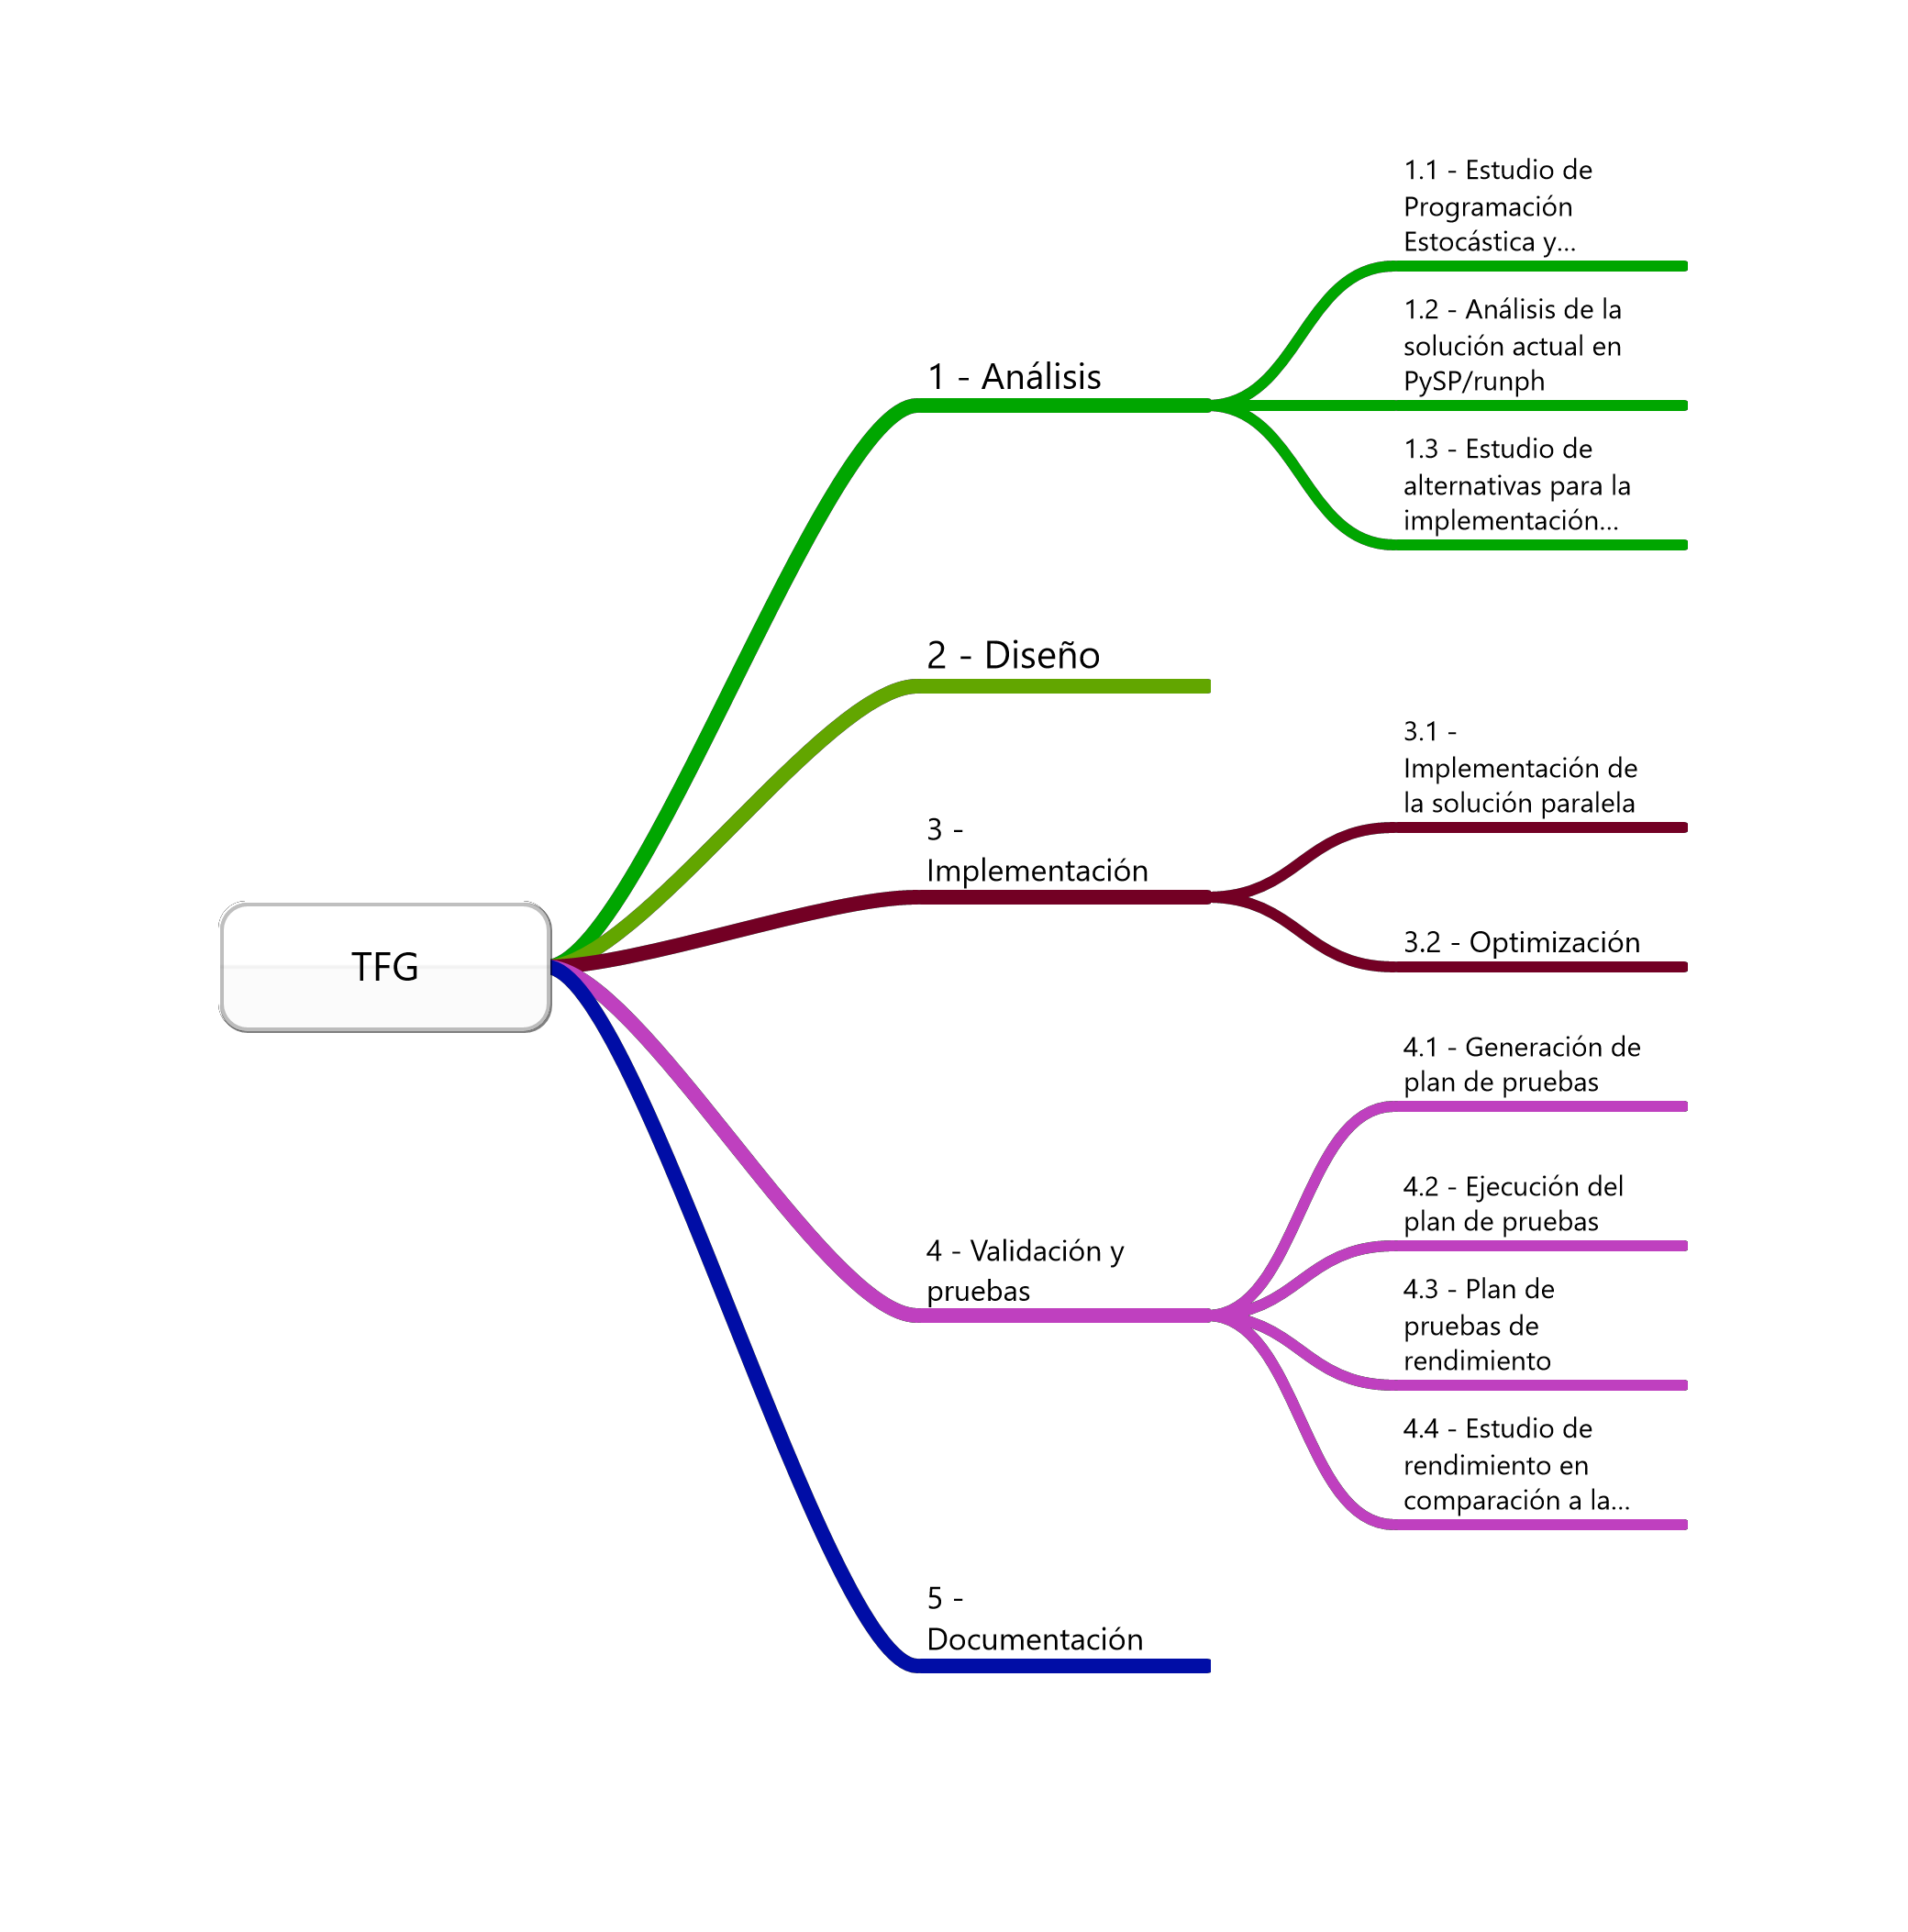
\includegraphics[width=15cm]{figuras/planificacion/edt-inicial.png}}
    \caption{EDT inicial}
\end{figure}

\WorkItem [
            id=1.1, 
            name={Estudio de Programación Estocástica y Progressive Hedging},
            duration=7,
            results={N/A}
        ]
{
    Se investigará el funcionamiento del algoritmo {\it Progressive Hedging} haciendo uso principalmente de \cite{stochasticProgramming} como referencia.
}

\WorkItem [
        id=1.2, 
        name={Análisis de la solución actual en PySP/runph},
        duration=8,
        results={Diagrama de funcionamiento PH \cite{local_funcionamientoPH}.}
    ]
{
    Una vez conocido el funcionamiento teórico del algoritmo, estudiar su implementación sobre el proyecto Pyomo.
}

\WorkItem [
        id=1.3, 
        name={Estudio de alternativas para la implementación paralela},
        duration=3,
        results={TODO}
    ]
{
    Se barajarán tecnologías Big Data (Spark) o modelos tradicionales (MPI).
}

\WorkItem [
        id=2, 
        name={Diseño},
        duration=20,
        results={Diseño de la implementación.}
    ]
{
    Generar un diseño de la implementación a realizar con la tecnología escogida. Será importante la integración con la implementación actual.
}

\WorkItem [
        id=3.1, 
        name={Implementación de la solución paralela},
        duration=15,
        results={Nuevos ficheros de código y modificaciones a archivos existentes.}
    ]
{
    Escribir los nuevos módulos de código e integrarlos en el proyecto. 
}

\WorkItem [
        id=3.2, 
        name={Optimización},
        duration=5,
        results={Modificaciones a la implementación anterior.}
    ]
{
    Una vez la integración es correcta y la implementación funciona, se realizarán optimizaciones de rendimiento intentando aprovechar las carácterísticas de la tecnología escogida para la nueva implementación paralela.
}

\WorkItem [
        id=4.1, 
        name={Generación de plan de pruebas},
        duration=4,
        results={Documento de pruebas \cite{local_planPruebas}.}
    ]
{
    Idear un plan de pruebas para el nuevo módulo.
}

\WorkItem [
        id=4.2, 
        name={Ejecución del plan de pruebas},
        duration=1,
        results={Informe de ejecución de pruebas.}
    ]
{
    Implementar y ejecutar las pruebas establecidas para establecer confianza sobre el correcto funcionamiento de la implementación.
}

\WorkItem [
        id=4.3, 
        name={Plan de pruebas de rendimiento},
        duration=3,
        results={Documento de pruebas de rendimiento \cite{local_planPruebasRendimiento}.}
    ]
{
    Idear un plan de pruebas con problemas que permitan estudiar el rendimiento del programa.
}

\WorkItem [
        id=4.4, 
        name={Estudio de rendimiento},
        duration=2,
        results={Informe de rendimiento \cite{local_informeRendimiento}.}
    ]
{
    Ejecutar el plan de pruebas anterior y compararlo con las versiones originales tanto secuencial como con Pyro.
}



\WorkItem [
        id=5, 
        name={Documentación},
        duration=10,
        results={Memoria del proyecto y documentos asociados.}
    ]
{
    Generar los documentos asociados al desarrollo del proyecto.
}

\subsubsection{Tareas no planificadas}



\subsection{Cronograma inicial}

Para la realización del trabajo se plantea un ciclo de vida en cascada. Este ciclo de vida nos permitirá realizar un seguimiento del progreso del proyecto en función del tiempo disponible.

\begin{figure}[H]
    \centerline{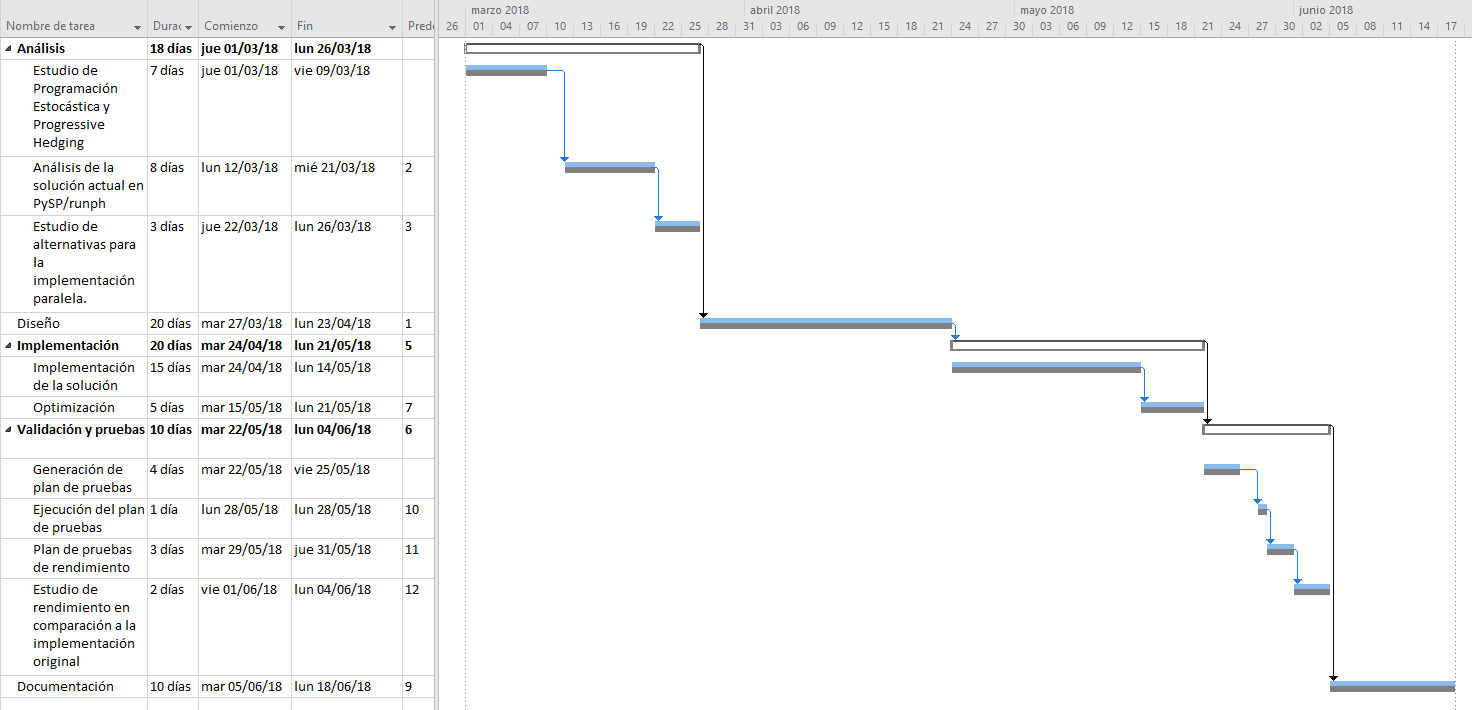
\includegraphics[width=15cm]{figuras/planificacion/linea-base.png}}
    \caption{Línea base}
\end{figure}

\subsection{Modificaciones al cronograma inicial}

Se ha realizado una estimación temporal inicial poco precisa por no utilizar ningún tipo de método probado ni datos concretos.

Esta es la razón principal para los fallos de cumplimiento de la planificación, al menos durante las fases de análisis y diseño.

El primer retraso se produce en la fase de análisis de la implementación actual. En esta fase se debe estudiar el funcionamiento del proyecto Pyomo y, en concreto, el módulo de resolución de problemas mediante Progressive Hedging. 

A pesar de conocer el funcionamiento teórico del algoritmo mediante \cite{}, Pyomo es un proyecto complejo, con multitud de funcionalidades para resolver otros tipos de problemas, soporte para plugins, etc. Todo esto hace que la complejidad del código aumente y sea necesario estudiar múltiples capas de abstracción para entender correctamente el funcionamiento del programa.

Otra complicación añadida es el personal desconocimiento del lenguaje Python previo a la realización de este trabajo.\\

Tras este primer retraso se intenta ajustar la planificación reduciendo el tiempo de diseño a la mitad:

\begin{figure}[H]
    \centerline{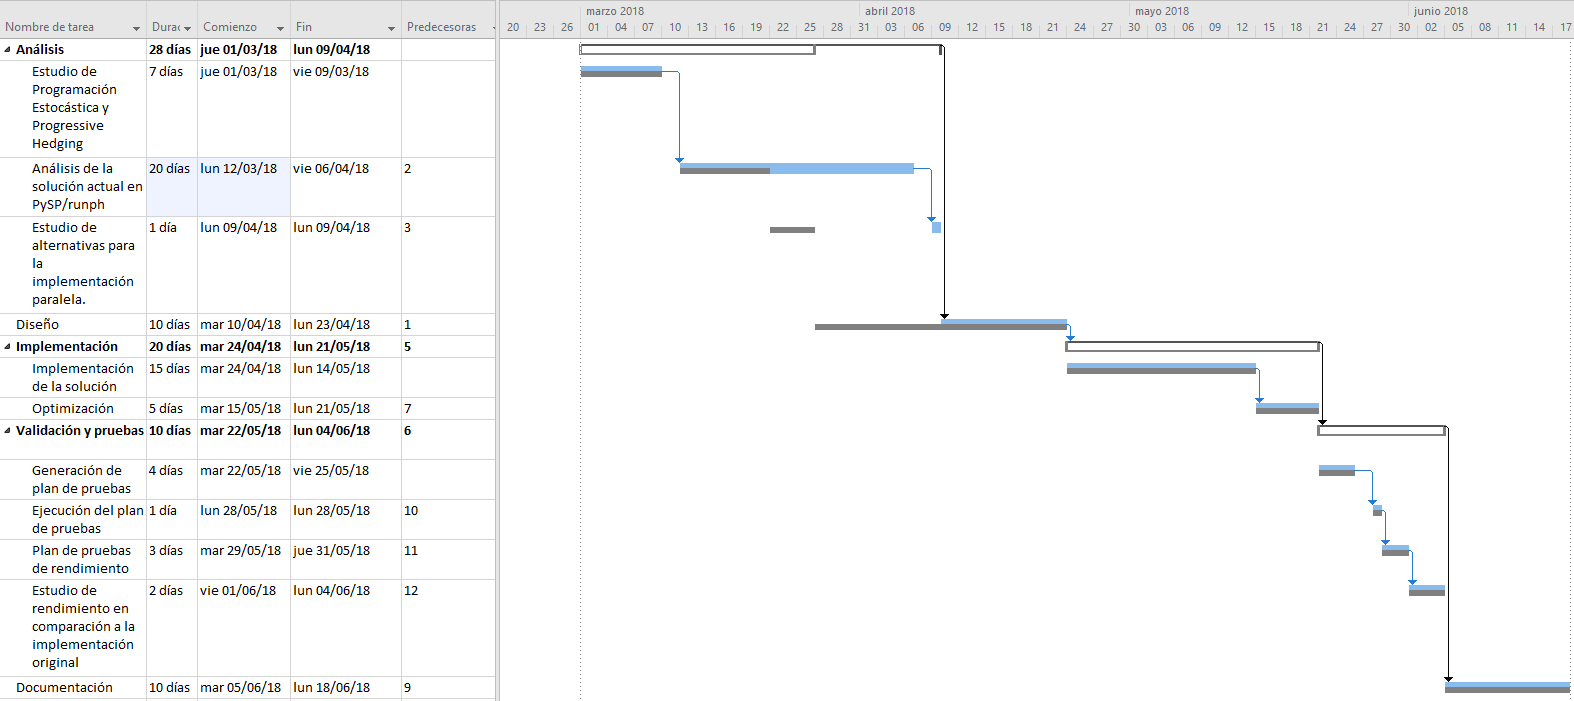
\includegraphics[width=15cm]{figuras/planificacion/1_retraso-analisis-inicial.png}}
    \caption{Primer retraso}
\end{figure}

Teniendo en cuenta que los primeros retrasos fueron principalmente causados por el desconocimiento de la tecnología a usar así como de una mala estimación, es muy probable que en las fases siguientes se produzcan otros retrasos. En este punto se considera entonces abandonar el ciclo de vida en cascada. Su principal atractivo era poder ajustarnos a una planificación temporal que nos permita acabar el proyecto dentro de tiempo, pero esta ventaja no se está cumpliendo en la práctica. Buscando reducir el tiempo de implementación con tecnologías que serán usadas por primera vez, se decide adaptar la planificación a un ciclo de vida por prototipos. 

La creación de sucesivos prototipos permite ir acostumbrándose a las tecnologías desconocidas, en este caso Python y Spark, así como ir probando el rendimiento y la integración a medida que se desarrolla.

En primer lugar se crea un prototipo aislado para comprobar la implementación de Spark con una arquitectura similar a la que se implementará en Pyomo. Este primer prototipo sirve como aprendizaje de la instalación de Spark y el despliegue de una aplicación en el mismo, así como la implementación en python que interactuará con Spark. Es deseable utilizar una arquitectura de objetos python similar a la que se usará en Pyomo para concretar el uso de Spark y descubrir posibles problemas con la implementación elegida.

Posteriormente se realizarán prototipos sucesivos sobre Pyomo para integrar el nuevo módulo e ir solucionando posibles problemas de rendimiento o funcionamiento que vayan surgiendo. 

Dado que la implementación partirá de un protipo inicial de baja calidad será importante realizar una fase de optimización y refactorización al final de la implementación para asegurarse un código final de calidad. Definir la calidad del código no es algo trivial y en este caso calificaremos el código como "de calidad" si cumple:
% TODO: meter mierdas de calidad de software y si eso alguna ISO

\begin{itemize}
    \item Funciona correctamente y es resistente a errores. Para esto nos apoyaremos en un plan de pruebas funcional.
    \item Funciona eficientemente y otorga un buen rendimiento, en comparación a las implementaciones existentes. En este caso nos apoyaremos en el plan de pruebas de rendimiento.
    \item Se integra adecuadamente al proyecto actual. Debe seguir una filosofía de diseño análoga al resto del código así como funcionar correctamente de forma paralela a todo lo implementado previamente.
\end{itemize}

Tras esta modificación en la planificación, se genera una nueva planificación que podemos ver en la figura y se guardará como una nueva línea base.% TODO

\begin{figure}[H]
    \centerline{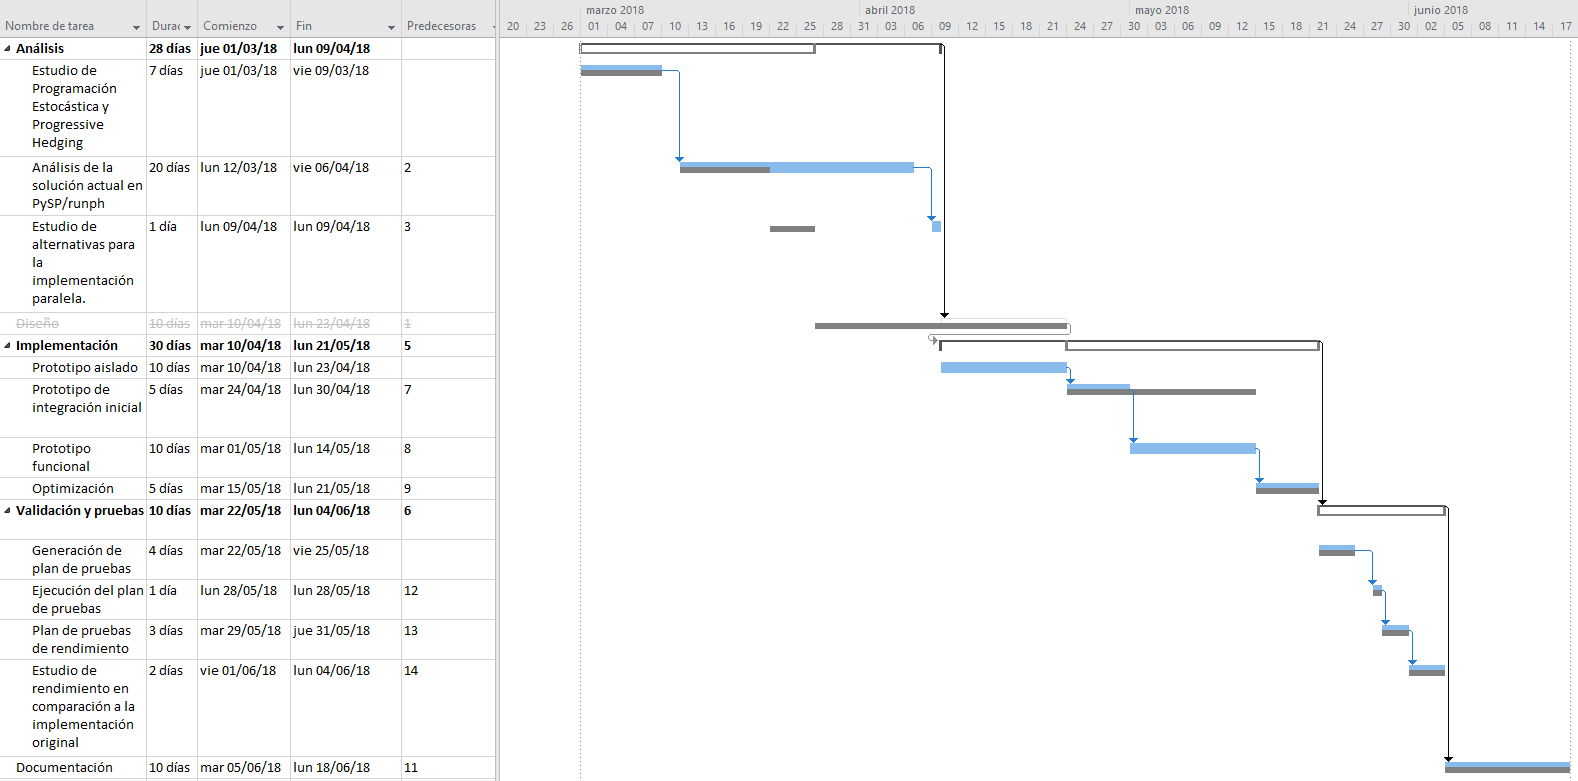
\includegraphics[width=15cm]{figuras/planificacion/2_linea-base-prototipos.png}}
    \caption{Línea base prototipos}
\end{figure}

En este punto hemos eliminado la fase de Diseño para poder aumentar el tiempo asignado a Análisis e Implementación. En caso de sufrir más retrasos en la fase de implementación podremos reducir el tiempo asignado a pruebas si el retraso no es grave. En caso de ser un retraso mayor, no cumpliremos la fecha de finalización establecida.

% TODO: Retrasos
% - Análisis se retrasa mucho porque el proyecto es complejo
% - Diseño se elimina y pasamos a hacerlo por prototipos porque así es más fácil adaptarse a Spark que es algo nuevo y es más sencillo ir integrándolo con Pyomo.
% - Implementación se retrasa porque está todo roto.
% - Plan de pruebas se hará a correr supongo
% - Se retrasa la fecha de finalización planificada.

